\documentclass[letterpaper]{article}
\usepackage{amssymb}
\usepackage{fullpage}
\usepackage{amsmath}
\usepackage{epsfig,float,alltt}
\usepackage{psfrag,xr}
\usepackage[T1]{fontenc}
\usepackage{url}
\usepackage{pdfpages}
%\includepdfset{pagecommand=\thispagestyle{fancy}}

%
%***********************************************************************
%               New Commands
%***********************************************************************
%
%
\newcommand{\rb}[1]{\raisebox{1.5ex}{#1}}
 \newcommand{\trace}{\mathrm{trace}}
\newcommand{\real}{\mathbb R}  % real numbers  {I\!\!R}
\newcommand{\nat}{\mathbb R}   % Natural numbers {I\!\!N}
\newcommand{\cp}{\mathbb C}    % complex numbers  {I\!\!\!\!C}
\newcommand{\ds}{\displaystyle}
\newcommand{\mf}[2]{\frac{\ds #1}{\ds #2}}
\newcommand{\book}[2]{{Luenberger, Page~#1, }{Prob.~#2}}
\newcommand{\spanof}[1]{\textrm{span} \{ #1 \}}
 \newcommand{\cov}{\mathrm{cov}}
 \newcommand{\E}{\mathcal{E}}
\parindent 0pt
%
%
%***********************************************************************
%
%               End of New Commands
%
%***********************************************************************
%
\begin{document}


\baselineskip=48pt  % Enforce double space

%\baselineskip=18pt  % Enforce 1.5 space

\setlength{\parskip}{.3in}
\setlength{\itemsep}{.3in}

\pagestyle{plain}

{\Large \bf
\begin{center}
Rob 501 Fall 2014\\
Lecture 23\\
Typeset by:  Ilsun Song\\
Proof-read by: Yunxiang Xu\\
Revised by Ni on 21 Nov. 2015
\end{center}
}


\Large

\begin{center}
    \textbf{Sequence}
\end{center}

\noindent \textbf{Def.}~ A set of vectors indexed by the non-negative integers is called a \underline{sequence} $(x_n)$ or $\{x_n\}$. Let $(x_n)$ be a sequence and $n_1<n_2<n_3<\dotsb $ be an infinite set of strictly increasing integers. Then, $(x_{n_i})$ is called a \underline{subsequence} of $(x_n)$.\\
    \underline{Example:}
    \begin{equation*}
        n_i = 2i + 1\textnormal{ or }n_i = 2^i
    \end{equation*}


\noindent \textbf{Def.}~ A sequence of vectors $(x_n)$ \underline{converges} to $x\in X$ if, $\forall$ ${\varepsilon} > 0,\ {\exists} N({\varepsilon}) < {\infty}$ such that, $n{\geq}N$, then ${\Vert}x_n-x{\Vert} < {\varepsilon}$, i.e., $n {\geq}N\Rightarrow \ x_n {\in} B_{\varepsilon}(x).$ One writes
    \begin{equation*}
        \lim\limits_{n \to \infty} x_n= x\textnormal{ or }x_n \rightarrow  x\textnormal{ or }x_n  \xrightarrow[n \to \infty]{} x.
    \end{equation*}

\noindent \textbf{Proposition:}~  Suppose $x_n \rightarrow x $. Then,
    \begin{enumerate}
        \item $\Vert x_n \Vert \rightarrow \Vert x \Vert$
        \item $\sup\limits_{n}\Vert x_n \Vert < \infty$ (The sequence is bounded.)
        \item If $x_n \rightarrow y$ then y = x. (Limits are unique.)
    \end{enumerate}

\noindent \textbf{Aside:}~ Useful inequality (Triangular inequality)\\
    For $\overline{x},\ \overline{y}\in X,$
    \begin{align*}
    &\ \ \ \ \ \Vert \overline{x} \Vert = \Vert \overline{x}-\overline{y}+\overline{y} \Vert \leq \Vert \overline{x}-\overline{y} \Vert + \Vert \overline{y} \Vert\\
        &\Rightarrow \Vert \overline{x} \Vert -\Vert \overline{y} \Vert \leq \Vert \overline{x}-\overline{y} \Vert\\
        &\therefore \vert \Vert \overline{x} \Vert - \Vert \overline{y} \Vert \vert \leq \Vert \overline{x}-\overline{y}\Vert
    \end{align*}

\noindent \underline{Proof:}
    \begin{enumerate}
        \item $\vert \Vert x \Vert - \Vert x_n\Vert\vert \leq \Vert x-x_n\Vert$ $\xrightarrow[n \to \infty]{}$ 0.
        \item Set $\varepsilon = 1$, $\exists N(1) <\infty$ such that $n \geq N,\ \|x_n-x\| \leq 1$.\\
            $\therefore$ $\forall$ $n \geq N,\ \Vert x_n\Vert =\|x_n-x+x\| \leq \Vert x_n - x\Vert + \Vert x \Vert \leq 1+\Vert x \Vert.$
            \begin{equation*}
                \sup\limits_{k}\Vert x_k\Vert \leq \operatorname{max}\{\underbrace{\Vert x_1\Vert, \Vert x_2\Vert, \dotsb , \Vert x_{n-1}\Vert, 1+ \Vert x \Vert}_\textnormal{finite}\}<\infty.
            \end{equation*}
        \item $\Vert x-y\Vert = \Vert x-x_n +x_n-y\Vert \leq \Vert x-x_n\Vert + \Vert x_n -y\Vert \xrightarrow[n \to \infty]{}$ 0.
    \end{enumerate}

\noindent \textbf{Def.}~ $x\in X$, P $\subset$ X a subset. $x$ is a \underline{limit point} of $P$ if $\exists$ a sequence of elements of $P$ that converges to $x$. That is, $\exists (x_n),\ x_n\in P,\ \textnormal{and} \lim\limits_{n \to \infty} x_n = x.$

\noindent \textbf{Proposition:}~ $x$ is a limit point of $P\Leftrightarrow x\in\overline{~P~}$.\\
    \underline{Proof:}
    \begin{enumerate}
        \item Suppose $x$ is a limit point. Then, $\exists (x_n)$ such that $x_n\in P$ and $x_n\rightarrow x$. Because $x_n\rightarrow x$, $\forall\varepsilon>0$, $\exists x_n\in P$ such that $\|x_n-x\|<\varepsilon$ $\Rightarrow$ $d(x,\ P)=0$ $\Rightarrow$ $x\in\overline{~P~}$.
        \item Suppose $x\in\overline{~P~}$. Then, $\forall$ $\varepsilon>0$, $\exists$ $y\in P$ such that $\|x-y\|<\varepsilon$. Let $\varepsilon=\frac{1}{n}$. Then, $\exists$ $x_n\in P$ such that $\|x-x_n\|<\frac{1}{n}$\\
        $\Rightarrow$ $x_n\rightarrow x$.\\
        $\therefore$ $x$ is a limit point.
    \end{enumerate}

\noindent \textbf{Corollary:}~ $P$ is closed $\Leftrightarrow$ it contains its limit points.

\begin{center}
    \textbf{Complete Spaces (Banach Spaces)}
\end{center}

\noindent \textbf{Def.}~ A sequence $(x_n)$ in $(\mathcal{X},\ \|\cdot\|)$ is a \underline{Cauchy sequence} if $\forall$ $\varepsilon >$ 0, $\exists N(\varepsilon)$ < $\infty$, such that $n,\ m \geq N\Rightarrow\Vert x_n - x_m\Vert < \varepsilon$.

\noindent \textbf{Notation:}~ $\|x_n-x_m\|\xrightarrow[n,\ m \to \infty]{}0$

\noindent \textbf{Proposition:}~ If $x_n\rightarrow x$, then $(x_n)$ is Cauchy.\\
    \underline{Proof:}~ Let $\varepsilon>0$ and choose $N<\infty$ such that $n\geq N\Rightarrow\|x_n-x\|<\frac{\varepsilon}{2}$. Then,     \begin{align*}
            \Vert x_n - x_m \Vert &= \Vert x_n - x + x - x_m \Vert\\
            &\leq \Vert x_n - x \Vert + \Vert x- x_m \Vert\\
            &< 0.5\varepsilon + 0.5\varepsilon\\
            &< \varepsilon\ \ \ \ \ \textnormal{for all }n,\ m\geq N\ \square
        \end{align*}
    Unfortunately, not all Cauchy sequences are convergent. For a reason we will understand shortly, all counter examples are infinite dimensional.\\ \\
    \underline{Example:}  $ X =  \{f:[0,1] \rightarrow \real \ \vert\ \textnormal{f continuous}\}$ and $ \Vert f \Vert_1 = \int_0^1 \vert f(\tau)\vert d\tau$.\\ \\
    Define a sequence as follow\\
    \begin{figure}[ht]
        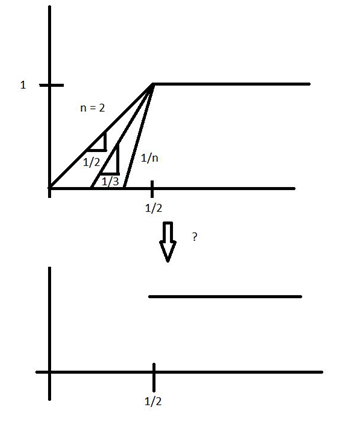
\includegraphics{typeset.png}
    \end{figure}
    $f_n(t)=\begin{cases}
        0 & 0\leq t\leq\frac{1}{2}-\frac{1}{n}\\
        1+n(t-\frac{1}{2}) & \frac{1}{2}-\frac{1}{n}\leq t\leq\frac{1}{2}\\
        1 & t\geq\frac{1}{2}
    \end{cases}
    $\\ \\
    $\Vert f_n - f_m \Vert_1=\frac{1}{2}$  $|\frac{1}{n}- \frac{1}{m}|$ $\xrightarrow[n,\ m \to \infty]{}$ 0, but there is no continuous $f$, such that $f_n \rightarrow f$.

\noindent \textbf{Def.}~ A normed space $(X,\real,\Vert\cdot\Vert)$ is \underline{complete} if every Cauchy Sequence in $X$ has a limit in $X$. Such spaces are called \underline{Banach spaces}.\\
    There are many useful and known Banach spaces.\\ \\
    In EECS562, you will use $\left(C\left[0,\ T\right],\ \|\cdot\|_\infty\right)$.

\noindent \textbf{Def.}~ A subset $P$ of a normed space is \underline{complete} if every Cauchy Sequence in $P$ has a limit in P.

\noindent \textbf{Remark:} $P$ is complete $\Rightarrow$ $P$ is closed.

\noindent \textbf{Theorem:}
    \begin{enumerate}
        \item In a normed linear space, any finite dimensional subspace is complete.
        \item Any closed subset of a complete set is also complete.
        \item $C\left[a,\ b\right]$, $\|\cdot\|_\infty$ is complete where $C\left[a,\ b\right]=\left\{f:\left[a,\ b\right]\rightarrow\real\ |\ f\textnormal{ continuous}\right\}$\\
        Note: $a<b$, both finite.
    \end{enumerate}

\end{document}















\end{document}
